\usetikzlibrary{mindmap,trees, backgrounds}
%\pagestyle{empty}
\begin{center}
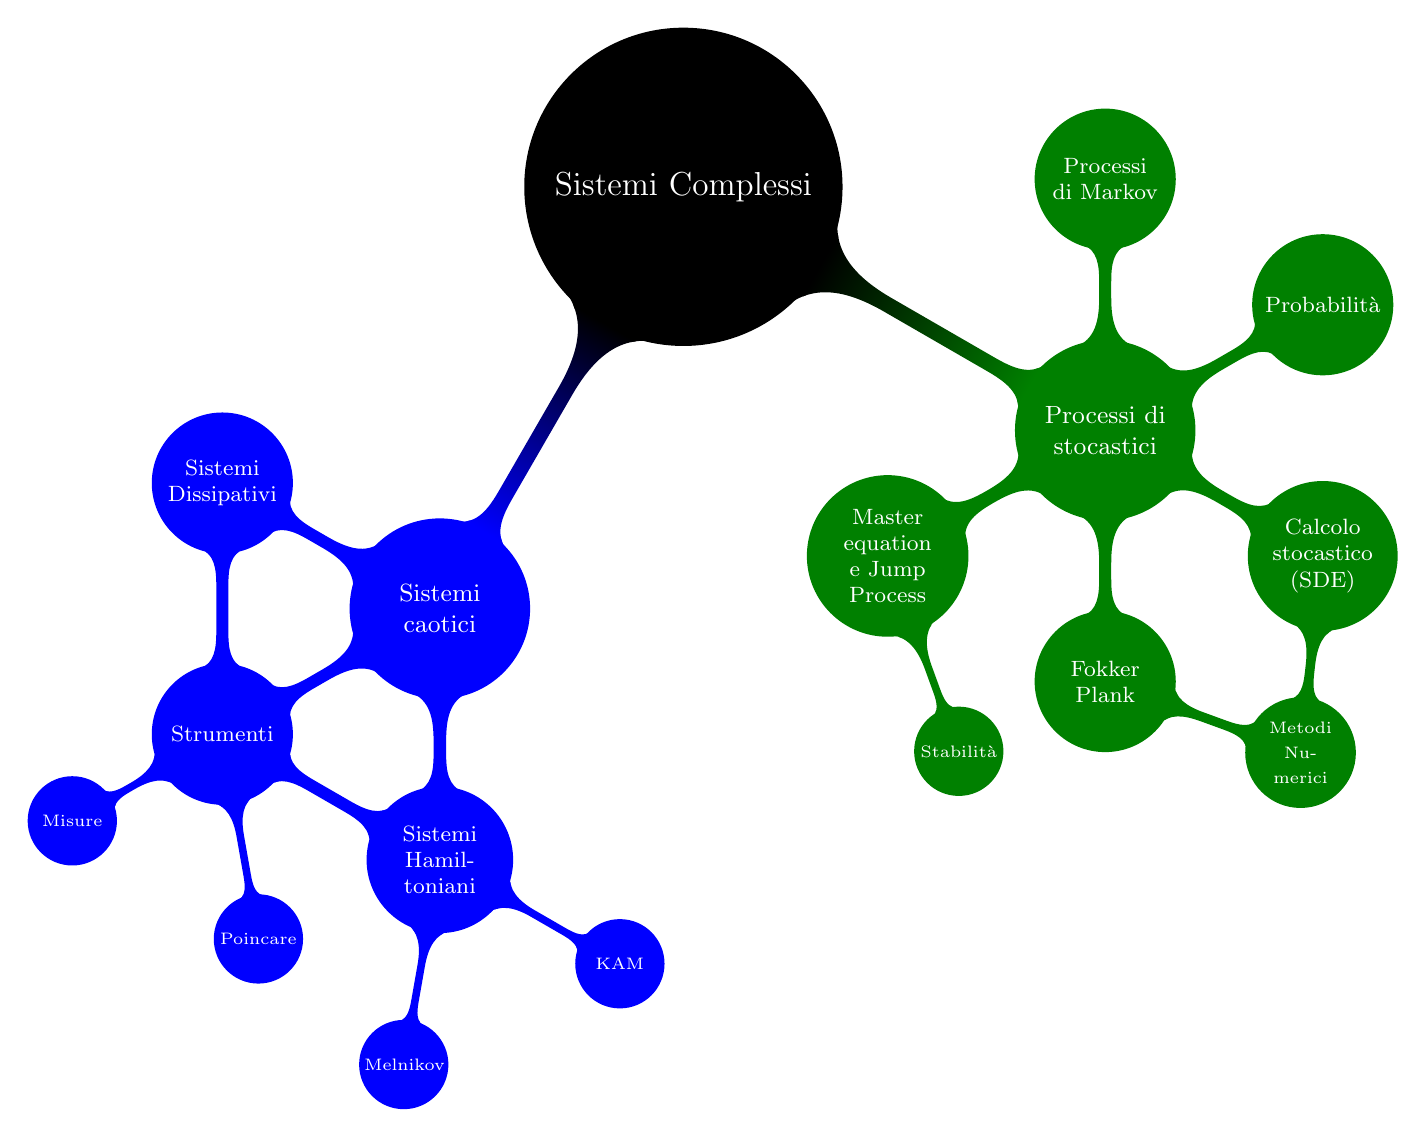
\begin{tikzpicture}
  \path[mindmap,
      concept color=black,
      text=white,
      level 1 concept/.append style={level distance=160,sibling angle=90, scale = 1.1},
      level 3 concept/.append style={sibling angle=70, minimum size=0.5cm,  font=\fontsize{6pt}{9pt}\selectfont}]
  node[concept] (main) {Sistemi Complessi}
    [clockwise from=-30]
    child[concept color=green!50!black] {
      node[concept] (stoc) {Processi di stocastici}
      [clockwise from=90]
      child { node[concept] (mark) {Processi di Markov} }
      child { node[concept] (prob) {Probabilità} }
      child { node[concept] (SDE) {Calcolo stocastico (SDE) } }
      child { node[concept] (FK) {Fokker Plank}
	[clockwise from=-20]
	child[concept color=green!50!black] {
	   node[concept] (num1) {Metodi Numerici}
      	}
      }
      child { node[concept] (master) {Master equation e Jump Process}
      	[clockwise from=-70]
	child[concept color=green!50!black] {
	   node[concept] (stab) {Stabilità}
      	}
      }
    }  
    child[concept color=blue] {
      node[concept] (caos) {Sistemi caotici}
      [clockwise from=-90]
      child { node[concept] (Ham) {Sistemi Hamiltoniani} 
	[clockwise from=-30]
	child[concept color=blue] { node[concept] (kam) {KAM} }
	child[concept color=blue] { node[concept] (mel) {Melnikov} }
      }
      child { node[concept] (strum) {Strumenti} 
	[clockwise from=-80]
	child[concept color=blue] { node[concept] (poin) {Poincare} }
	child[level distance=2cm, concept color=blue] { node[concept] (mel) {Misure} }
      }
      child { node[concept] (diss) {Sistemi Dissipativi} }
    };
    \begin{pgfonlayer}{background}
	\draw (num1) to[circle connection bar switch color=from (green!50!black) to (green!50!black)] (SDE);
	\draw (strum) to[circle connection bar switch color=from (blue) to (blue)] (diss);
	\draw (strum) to[circle connection bar switch color=from (blue) to (blue)] (Ham);
    \end{pgfonlayer}
\end{tikzpicture}
\end{center}
